% !TEX root = ../FundationsDataScience.tex

\chapter{Deep Learning}
\label{c-deep-learning}

% Ref: \cite{Rufflewind2017blog}

Before detailing deep architectures and their use, we start this chapter by presenting two essential computational tools that are used to train these model: stochastic optimization methods and automatic differentiation. In practice, they work hand-in-hand to be able to learn painlessly complicated non-linear models on large-scale datasets. 


%%%%%%%%%%%%%%%%%%%%%%%%%%%%%%%%%%%%%%%%%%%%%%%%%%%%%%%%%%%%%%%%%%%%%%%%
%%%%%%%%%%%%%%%%%%%%%%%%%%%%%%%%%%%%%%%%%%%%%%%%%%%%%%%%%%%%%%%%%%%%%%%%
%%%%%%%%%%%%%%%%%%%%%%%%%%%%%%%%%%%%%%%%%%%%%%%%%%%%%%%%%%%%%%%%%%%%%%%%
\section{Stochastic Optimization}
\label{sec-stochastic-optim}

We detail some important stochastic Gradient Descent methods, which enables to perform optimization in the setting where the number of samples $n$ is large and even infinite. 

% We set the classes indexes to be $\{-1,+1\}$, and remove empty features, normalize $X$. $n$ is the number of samples, $p$ is the dimensionality of the features,

%%%%%%%%%%%%%%%%%%%%%%%%%%%%%%%%%%%%%%%%%%%%%%%%%%%%%%%%
\subsection{Minimizing Sums and Expectation}

A large class of functionals in machine learning can be expressed as minimizing large sums of the form
\eql{\label{eq-min-sums}
	\umin{\be \in \RR^p} \Ee(\be) \eqdef \frac{1}{n} \sum_{i=1}^n \Ee_i(\be)
}
or even expectations of the form
\eql{\label{eq-min-int}
	\umin{\be \in \RR^p}  \Ee(\be) \eqdef \EE_{\zp \sim \pi}( f(\be,\zp) ) = \int_{\Zz} \Ee(\be,z) \d\pi(z).
}
Problem~\eqref{eq-min-sums} can be seen as a special case of~\eqref{eq-min-int}, when using a discrete empirical uniform measure $\pi = \sum_{i=1}^n \de_i$ and setting $\Ee(x,i)=\Ee_i(x)$. One can also viewed~\eqref{eq-min-sums} as a discretized ``empirical'' version of~\eqref{eq-min-int} when drawing $(z_i)_i$ i.i.d. according to $\zp$ and defining $\Ee_i(x)=\Ee(x,z_i)$. In this setup,~\eqref{eq-min-sums} converges to~\eqref{eq-min-int} as $n \rightarrow +\infty$.

A typical example of such a class of problems is empirical risk minimization (here without regularization $J=0$ for simplicity)~\eqref{eq-erm-param} and its expectation version~\eqref{eq-consistency-param}, where in these cases
\eql{\label{eq-stochastic-erm}
	\Ee_i(\be) = \loss(f(x_i,\be),y_i)
	\qandq
	\Ee_i(\be,z) = \loss(f(x,\be),y)
}
for $z=(x,y) \in \Zz = (\Xx=\RR^p) \times (\Yy=\RR^q)$ (typically $q=1$). 
%
We illustrate bellows the methods on binary logistic classification, where
\eql{\label{eq-stoch-logistic}
	\loss(s,y ) \eqdef \log( 1+\exp(-sy) ) \qandq f(x,\be) = \dotp{x}{\be}, 
}
see Section~\ref{sec-two-class-logit}�for details. But this extends to arbitrary parametric models, and in particular deep neural networks as detailed in Section~\ref{sec-deepnet-discr}. 

While some algorithms (in particular batch gradient descent) are specific to finite sums~\eqref{eq-min-sums}, the stochastic methods we detail next work verbatim (with the same convergence guarantees) in the expectation case~\eqref{eq-min-int}. For the sake of simplicity, we however do the exposition for the finite sums case, which is sufficient in the vast majority of cases. But one should keep in mind that $n$ can be arbitrarily large, so it is not acceptable in this setting to use algorithms whose complexity per iteration depend on $n$.

The general idea underlying stochastic optimization methods is \textit{not} to have faster algorithms with respect to traditional optimization schemes such as those detailed in Chapter~\ref{chap-conv-duality}. In almost all cases, if $n$ is not too large so that one afford the price of doing a few non-stochastic iterations, then deterministic methods are faster. But if $n$ is so large that one cannot do even a single deterministic iteration, then stochastic methods allow one to have a fined grained scheme by breaking the cost of determinstic iterations in smaller chunks. Another advantage is that they are quite easy to parallelize. 


%%%%%%%%%%%%%%%%%%%%%%%%%%%%%%%%%%%%%%%%%%%%%%%%%%%%%%%%
\subsection{Batch Gradient Descent (BGD)}

The usual deterministic (batch) gradient descent (BGD) is studied in details in Section~\ref{eq-general-pbm}. Its iterations read
\eq{
	\iit{\be} = \it{\be} - \tau_\ell \nabla \Ee(\it{\be})
}
and the step size should be chosen as $0 < \tau_{\min} < \tau_\ell < \tau_{\max} \eqdef 2/L$ where $L$ is the Lipschitz constant of the gradient $\nabla \Ee$. In particular, in this determinstic setting, this step size should not go to zero and this ensures quite fast convergence (even linear rates if $\Ee$ is strongly convex).

The computation of the gradient in our setting reads
\eql{\label{eq-full-grad}
	\nabla \Ee(\be) = \frac{1}{n} \sum_{i=1}^n \nabla \Ee_i(\be)
}
so it typically has complexity $O(np)$ if computing $\nabla f_n$ has linear complexity in $p$.

In the ERM setting~\eqref{eq-stochastic-erm}, the gradient reads 
\eql{\label{eq-grad-formula}
	\nabla \Ee_i(\be) = [\partial f(x_i,\be)]^\top ( \nabla \loss( f(x_i,\be),y_i ) ),
}
where $\partial f(x,\be) \in \RR^{q \times p}$ is the Jacobian of the mapping $\be \in \RR^p \mapsto f(x,\be) \in \RR^q$, while
$\nabla \loss( y,y' ) \in \RR^q$ is the gradient with respect to the first variable, i.e. the gradient of the map $y \in \RR^q \mapsto \loss(y,y') \in \RR$.

In the case of a linear model such as~\eqref{eq-stoch-logistic}, this gradient computation simply reads
\eq{
	\nabla \Ee_i(\be) = \loss'( \dotp{x_i}{\be}, y_i ) ) x_i 
}
where $\loss'$ is the differential of $\loss$ with respect to the first variable. For the logistic loss, it is simply 
\eq{
	\loss'(s,y) = -s \frac{e^{-sy}}{ 1+e^{-sy} }.
}


\begin{figure}
\centering
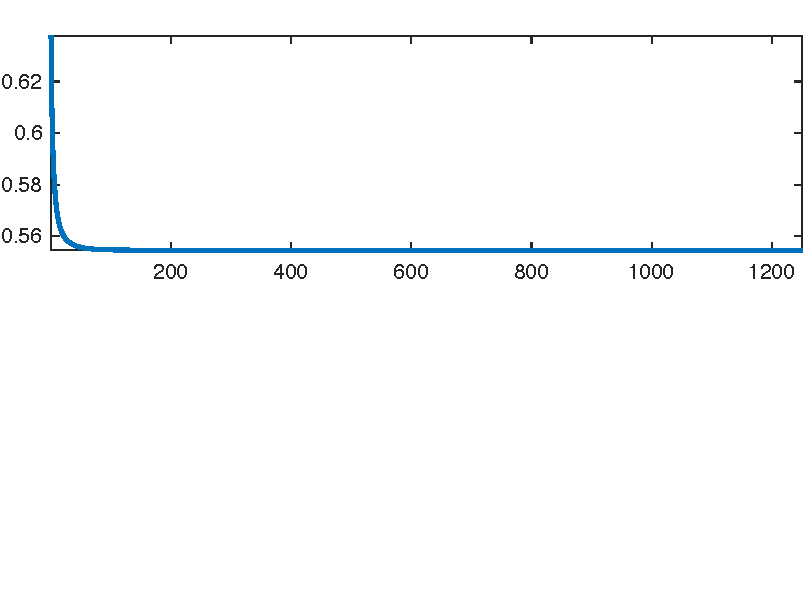
\includegraphics[width=.6\linewidth]{ml/sgd/error-bgd-1} \\
$\Ee(\it{\be})$ \\
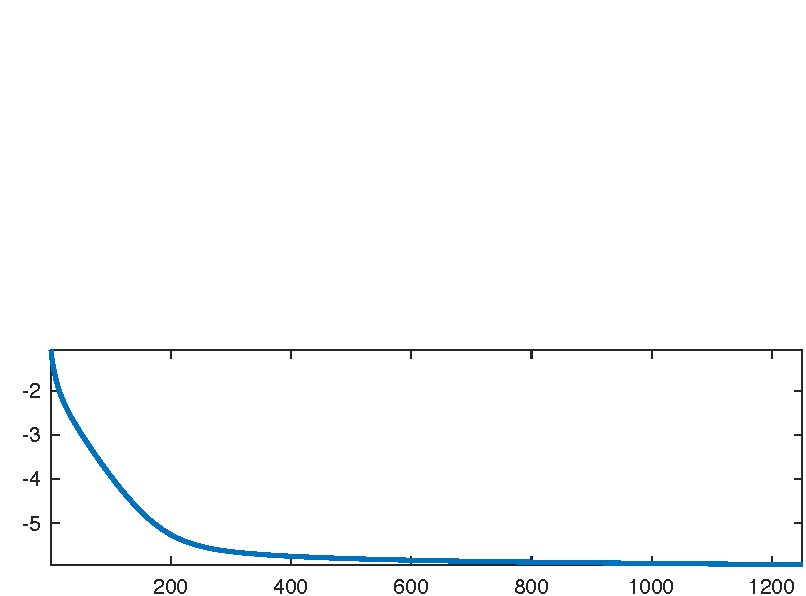
\includegraphics[width=.6\linewidth]{ml/sgd/error-bgd-2} \\
$\log_{10}(\Ee(\it{\be})-\Ee(\be^\star))$ 
\caption{\label{fig-bgd}
Evolution of the error of the BGD for logistic classification.
}
\end{figure}



%%%%%%%%%%%%%%%%%%%%%%%%%%%%%%%%%%%%%%%%%%%%%%%%%%%%%%%%
\subsection{Stochastic Gradient Descent (SGD)}

\wrapf{ml/sgd/unbiased-grad}{Unbiased gradient estimate}
For very large $n$, computing the full gradient $\nabla \Ee$ as in~\eqref{eq-full-grad} is prohibitive.  
%
The idea of SGD is to trade this exact full gradient by an inexact proxy using a single functional $\Ee_{i}$ where is drawn uniformly at random. The main idea that makes this work is that this sampling scheme provides an unbiased estimate of the gradient, in the sense that
\eql{\label{eq-unbiased-grad}
	\EE_{\ip}{ \nabla \Ee_{\ip}(\be) } = \nabla \Ee(\be)
}
where $\ip$ is a random variable distributed uniformly in $\{1,\ldots,n\}$.

\wrapf{ml/sgd/sgd-schematic}{Schematic view of SGD iterates}
Starting from some $\be^{(0)}$,the iterations of stochastic gradient descent (SGD) read
\eq{
	\iit{\be} = \it{\be} - \tau_\ell \nabla \Ee_{i(\ell)}(\it{\be})
}
where, for each iteration index $\ell$, $i(\ell)$
is drawn uniformly at random in $\{1,\ldots,n\}$. 
%
It is important that the iterates $\iit{\be}$ are thus random vectors, and the theoretical analysis of the method thus studies wether this sequence of random vectors converges (in expectation or in probability for instance) toward a deterministic vector (minimizing $\Ee$), and at which speed. 

Note that each step of a batch gradient descent has complexity $O(np)$,
while a step of SGD only has complexity $O(p)$. SGD is thus
advantageous when $n$ is very large, and one cannot afford to do
several passes through the data. In some situation, SGD can provide
accurate results even with $\ell \ll n$, exploiting redundancy between
the samples.

A crucial question is the choice of step size schedule $\tau_\ell$. It
must tends to 0 in order to cancel the noise induced on the gradient by
the stochastic sampling. But it should not go too fast to zero in order
for the method to keep converging. 


A typical schedule that ensures both properties is to have asymptotically $\tau_\ell \sim \ell^{-1}$ for
$\ell\rightarrow +\infty$. We thus propose to use 
\eql{\label{eq-stepsize-sgd}
	\tau_\ell \eqdef \frac{\tau_0}{1 + \ell/\ell_0}
}
where $\ell_0$ indicates roughly the number of iterations serving as a
``warmup'' phase.

Figure~\eqref{fig-sgd-traject} shows a simple 1-D example to minimize $f_1(\be)+f_2(\be)$ for $\be \in \RR$ and $f_1(\be)=(\be-1)^2$ and $f_2(\be)=(\be+1)^2$. One can see how the density of the distribution of $\it{\be}$ progressively clusters around the minimizer $\be^\star=0$. Here the distribution of $\be^{(0)}$ is uniform on $[-1/2,1/2]$.

\begin{figure}
\centering
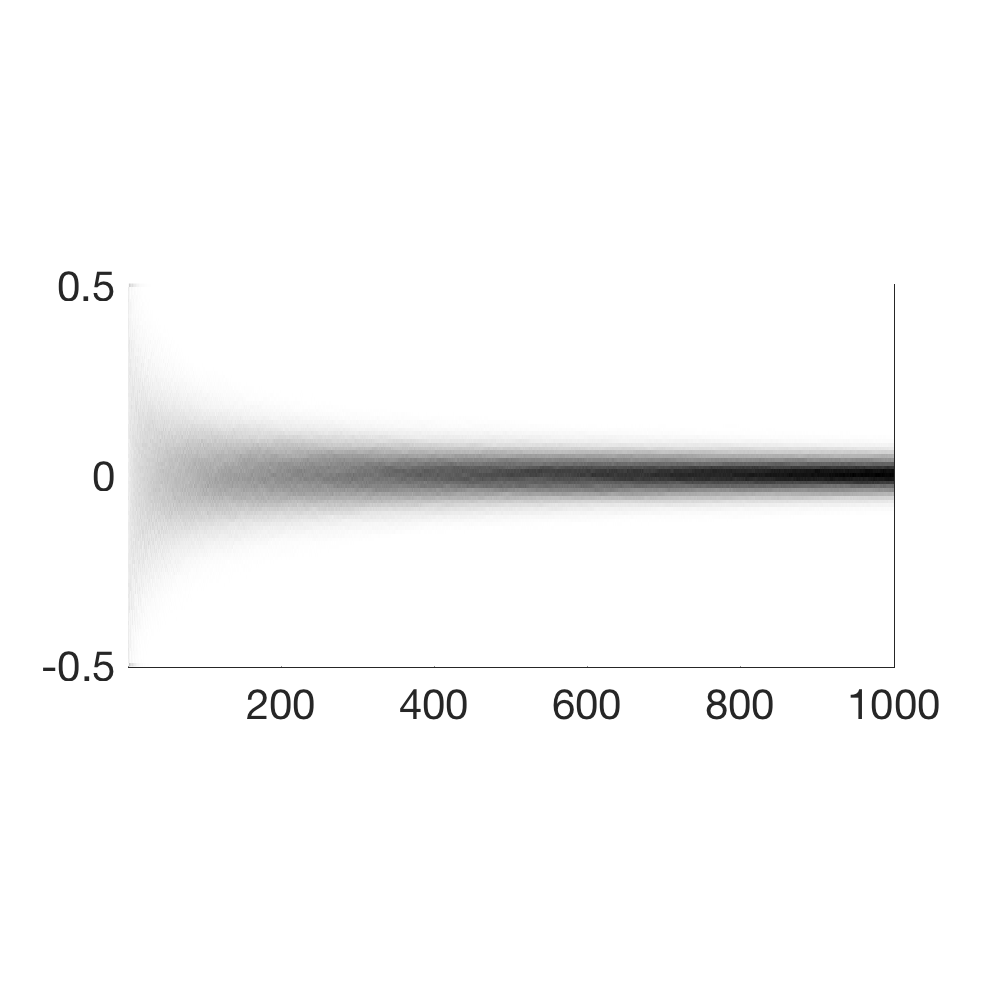
\includegraphics[width=.49\linewidth]{ml/sgd/sgd-histo} 
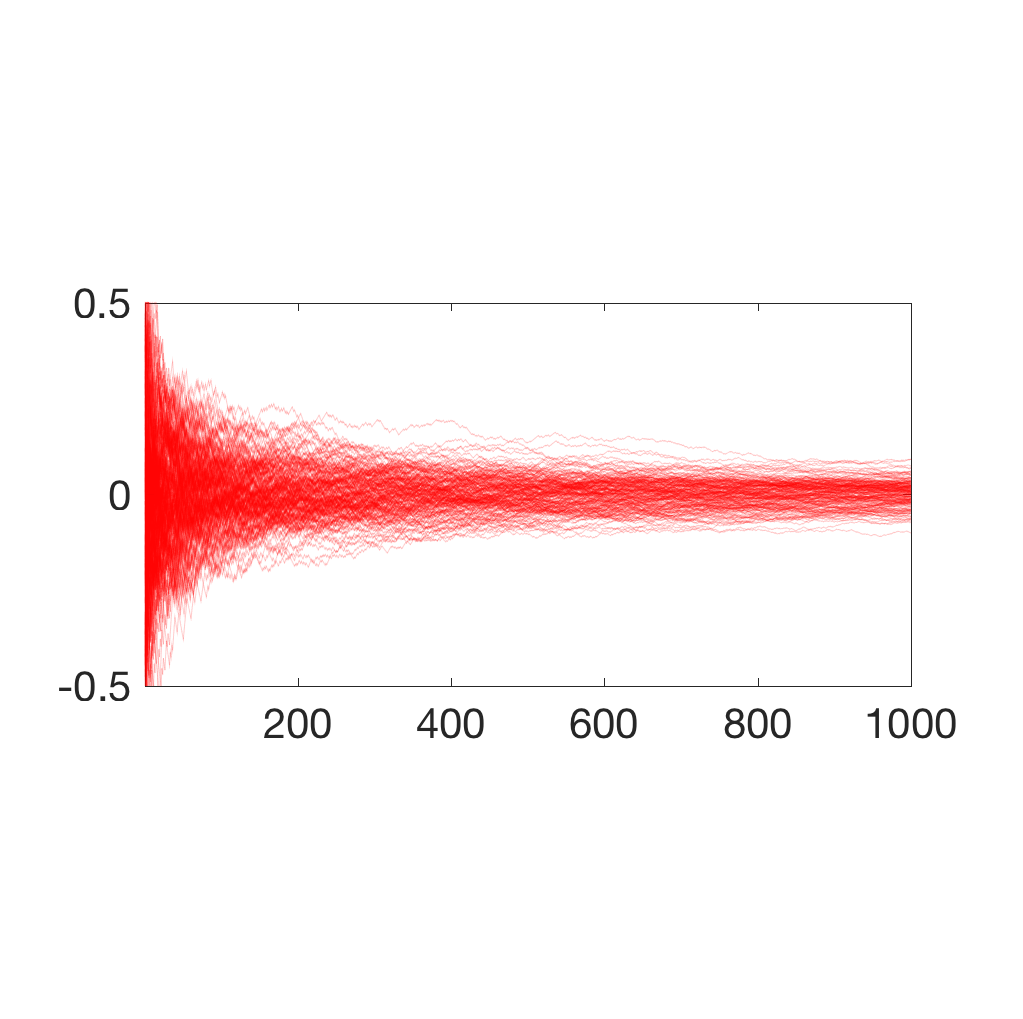
\includegraphics[width=.49\linewidth]{ml/sgd/sgd-trajectory}
\caption{\label{fig-sgd-traject}
Display of a large number of trajectories $\ell \mapsto \it{\be} \in \RR$ generated by several runs of SGD. On the top row, each curve is a trajectory, and the bottom row displays the corresponding density.
}
\end{figure}


The following theorem shows the convergence in expectration with a $1/\sqrt{\ell}$ rate on the objective.

\begin{thm}\label{thm-conv-sgd}
We assume $\Ee$ is $\mu$-strongly convex, and is such that $\norm{\nabla \Ee_i(x)}^2 \leq C^2$. 
For the step size choice $\tau_\ell = \frac{1}{\mu (\ell+1)}$, one has
\eql{\label{eq-rate-sgd}
	\EE( \norm{\it{\be}-\be^\star}^2 ) \leq \frac{ R }{\ell+1}
	\qwhereq
	 R = \max( \norm{\be^{(0)} - \be^\star}, C^2/\mu^2 ), 
}
where $\EE$ indicates an expectation with respect to the i.i.d.
sampling performed at each iteration.
\end{thm}

\begin{proof}
	By strong convexity, one has
	\begin{align*}
		\Ee(\be^\star) - \Ee(\it{\be}) &\geq \dotp{ \nabla\Ee(\it{\be}) }{ \be^\star-\it{\be} } + \frac{\mu}{2}\norm{\it{\be}-\be^\star}^2 \\
		\Ee(\it{\be}) - \Ee(\be^\star) &\geq \dotp{ \nabla\Ee(\be^\star) }{ \it{\be} - \be^\star } + \frac{\mu}{2}\norm{\it{\be}-\be^\star}^2.
	\end{align*}
	Summing these two inequalities and using $\nabla\Ee(\be^\star)=0$ leads to
	\eql{\label{eq-sgd-proof-1}
		\dotp{ \nabla\Ee(\it{\be}) - \nabla\Ee(\be^\star) }{ \be^\star-\it{\be} }
		=
		\dotp{ \nabla\Ee(\it{\be})  }{ \be^\star-\it{\be} }
		\geq \mu \norm{\it{\be}-\be^\star}^2.
	}
	Considering only the expectation with respect to the ransom sample of $i(\ell) \sim \ip_\ell$, one has
	\begin{align*}
		\EE_{\ip_\ell}( \norm{\iit{\be}-\be^\star}^2 )
		&= 
		\EE_{\ip_\ell}( \norm{\it{\be} - \tau_\ell \nabla \Ee_{\ip_\ell}(\it{\be}) -\be^\star}^2 ) \\
		&= 
		\norm{\it{\be} - \be^\star}^2 + 2\tau_\ell \dotp{ \EE_{\ip_\ell}(\nabla \Ee_{\ip_\ell}(\it{\be})) }{ \it{\be} -\be^\star } + 
			\tau_\ell^2  \EE_{\ip_\ell}( \norm{\nabla \Ee_{\ip_\ell}(\it{\be})}^2 ) \\
		&=
		\norm{\it{\be} - \be^\star}^2 + 2\tau_\ell \dotp{ \nabla \Ee(\it{\be})) }{ \it{\be} -\be^\star } + \tau_\ell^2 C^2 \\
	\end{align*}
	where we used the fact~\eqref{eq-unbiased-grad}�that the gradient is unbiased. 
	%
	Taking now the full expectation with respect to all the other previous iterates, and using~\eqref{eq-sgd-proof-1} one obtains
	\eql{\label{eq-sgd-proof-2}
		\EE( \norm{\iit{\be}-\be^\star}^2 ) \leq \EE( \norm{\it{\be} - \be^\star}^2 ) - 2 \mu \tau_\ell \EE( \norm{\it{\be} - \be^\star}^2 ) + \tau_\ell^2 C^2
		= (1-2 \mu \tau_\ell)  \EE( \norm{\it{\be} - \be^\star}^2 ) + \tau_\ell^2 C^2.
	}
	We show by recursion that the bound~\eqref{eq-rate-sgd} holds. We denote $\epsilon_\ell \eqdef \EE( \norm{\be^{(\ell)}-\be^\star}^2 )$.
	%
	Indeed, for $\ell=0$, this it is true that 
	\eq{
		\epsilon_0 \leq \frac{ \max( \norm{\be^{(0)} - \be^\star}, C^2/\mu^2 ) }{1} = \frac{R}{1}.
	}
	We now assume that $\epsilon_\ell \leq \frac{R}{\ell+1}$. Using~\eqref{eq-sgd-proof-2} in the case of $\tau_\ell = \frac{1}{\mu (\ell+1)}$, one has, denoting $m=\ell+1$
	\begin{align*}
		\epsilon_{\ell+1} &\leq (1-2 \mu \tau_\ell) \epsilon_\ell + \tau_\ell^2 C^2 = 
			\pa{1-\frac{2}{m}} \epsilon_\ell + \frac{C^2}{(\mu m)^2}  \\  
			&\leq
			\pa{1-\frac{2}{m}} \frac{R}{m} + \frac{R}{m^2}  = 
			\pa{ \frac{1}{m}-\frac{1}{m^2} } R
			= 
			\frac{m-1}{m^2} R
			= 
			\frac{m^2-1}{m^2}\frac{1}{m+1} R
			\leq
			\frac{R}{m+1}
	\end{align*}
\end{proof}

A weakness of SGD (as well as the SGA scheme studied next) is that it only weakly benefit from strong convexity of $\Ee$. This is in sharp contrast with BGD, which enjoy a fast linear rate for strongly convex functionals, see Theorem~\ref{thm-gradsec-non-strong-conv}.

Figure~\ref{fig-sgd} displays the evolution of the energy $\Ee(\it{\be})$. 
It overlays on top (black dashed curve) the convergence of the batch gradient descent, with a careful scaling of the 
number of iteration to account for the fact that the complexity of a batch iteration is $n$ times larger. 


\begin{figure}
\centering
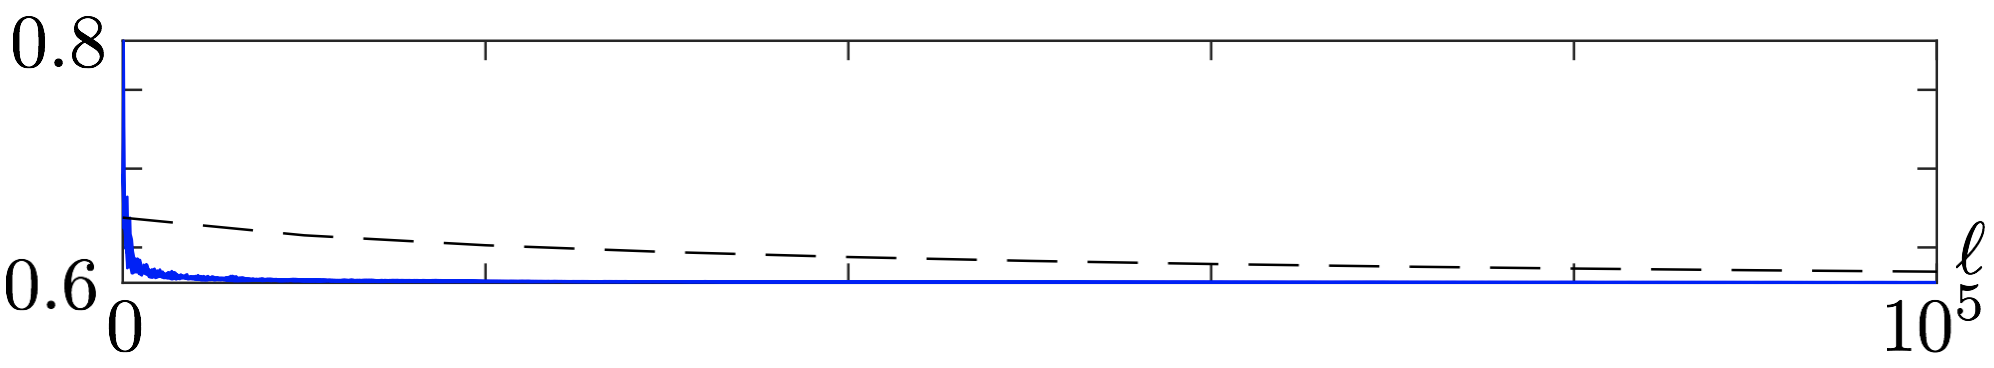
\includegraphics[width=.6\linewidth]{ml/sgd/error-sgd-1} \\
$\Ee(\it{\be})$ \\
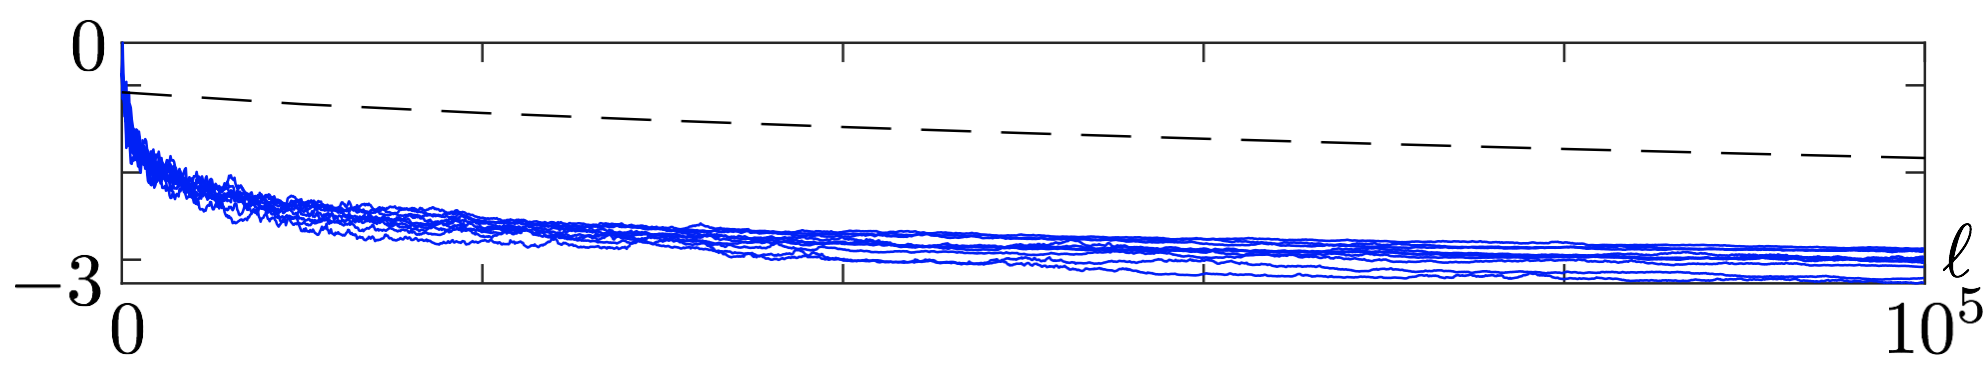
\includegraphics[width=.6\linewidth]{ml/sgd/error-sgd-2} \\
$\log_{10}(\Ee(\it{\be})-\Ee(\be^\star))$ 
\caption{\label{fig-sgd}
Evolution of the error of the SGD for logistic classification (dashed line shows BGD).
}
\end{figure}




%%%%%%%%%%%%%%%%%%%%%%%%%%%%%%%%%%%%%%%%%%%%%%%%%%%%%%%%
\subsection{Stochastic Gradient Descent with Averaging (SGA)}
\label{sec-sga}

Stochastic gradient descent is slow because of the fast decay of
$\tau_\ell$ toward zero.
%
To improve somehow the convergence speed, it is possible to average the past
iterate, i.e. run a ``classical" SGD on auxiliary variables $( \it{\tilde\be})_\ell$
\eq{
	 \iit{\tilde\be} = \it{\tilde\be} - \tau_\ell \nabla \Ee_{i(\ell)}(\it{\tilde\be})
}
and output as estimated weight vector the Cesaro average
\eq{
	\it{\be} \eqdef \frac{1}{\ell} \sum_{k=1}^\ell \it{\tilde\be}.
}
This defines the Stochastic Gradient Descent with Averaging (SGA)
algorithm.

Note that it is possible to avoid explicitly storing all the iterates by simply
updating a running average as follow
\eq{
	\iit{\be} = \frac{1}{\ell} \it{\tilde\be} +  \frac{\ell-1}{\ell} \it{\be}. 
}


In this case, a typical choice of decay is rather of the form 
\eq{
	\tau_\ell \eqdef \frac{\tau_0}{1 + \sqrt{\ell/\ell_0}}.
}
Notice that the step size now goes much slower to 0, at rate $\ell^{-1/2}$.


Typically, because the averaging stabilizes the iterates, the choice of
$(\ell_0,\tau_0)$ is less important than for SGD. 

% <https://arxiv.org/pdf/1303.6149.pdf 

Bach proves that for logistic classification, 
it leads to a faster convergence (the constant involved are
smaller) than SGD, since 
on contrast to SGD, SGA is adaptive to the local strong convexity of $E$.



%%%%%%%%%%%%%%%%%%%%%%%%%%%%%%%%%%%%%%%%%%%%%%%%%%%%%%%%
\subsection{Stochastic Averaged Gradient Descent (SAG)}

% https://arxiv.org/pdf/1309.2388
For problem size $n$ where the dataset (of size $n \times p$) can
fully fit into memory, it is possible to further improve the SGA method
by bookkeeping the previous gradients. This gives rise to the 
Stochastic Averaged Gradient Descent (SAG) algorithm.

We store all the previously computed gradients in $(G^i)_{i=1}^n$,
which necessitates $O(n \times p)$ memory. 
The iterates are defined by using a proxy $g$ for the batch gradient,
which is progressively enhanced during the iterates.

The algorithm reads
\eq{
	h \leftarrow \nabla \Ee_{i(\ell)}(\it{\tilde\be}),
}
\eq{
	g  \leftarrow g - G^{i(\ell)} + h,  
}
\eq{
	G^{i(\ell)} \leftarrow h, 
}
\eq{
	\iit{\be} = \it{\be} - \tau g. 
}
Note that in contrast to SGD and SGA, this method uses a fixed step
size $\tau$. Similarly to the BGD, in order to ensure convergence, 
the step size $\tau$ should be of the order of $1/L$
where $L$ is the Lipschitz constant of $\Ee$.

This algorithm improves over SGA and SGD
since it has a convergence rate of $O(1/\ell)$ as does BGD. 
Furthermore, in the presence of strong convexity (for instance when $X$ is
injective for logistic classification), it has a linear convergence rate, 
i.e. 
 \eq{
	\EE( \Ee(\it{\be}) ) - \Ee(\be^\star) = O\pa{ \rho^\ell },
}
for some $0 < \rho < 1$. 

Note that this improvement over SGD and SGA is made possible only because
SAG explicitly uses the fact that $n$ is finite (while SGD and SGA can
be extended to infinite $n$ and more general minimization of
expectations~\eqref{eq-min-int}).

Figure~\ref{fig-bgd} shows a comparison of SGD, SGA and SAG.

\begin{figure}
\centering
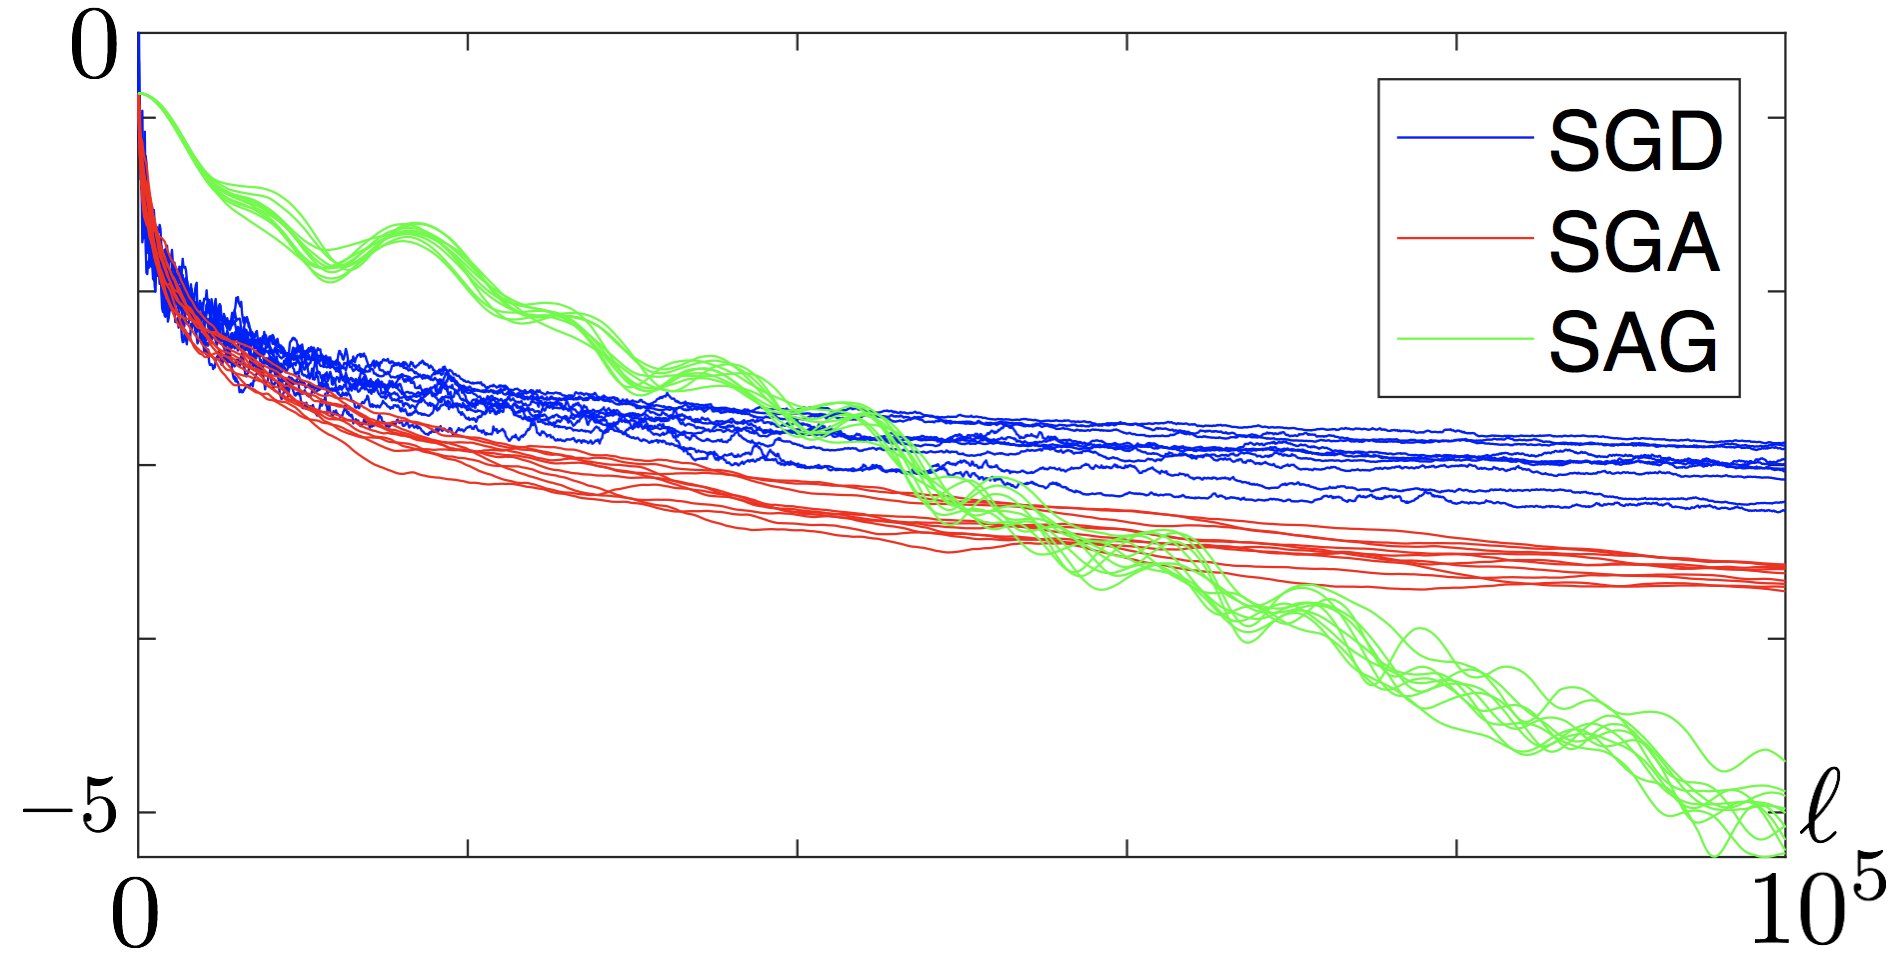
\includegraphics[width=.6\linewidth]{ml/sgd/sg-comparison}
\caption{\label{fig-bgd}
Evolution of $\log_{10}(\Ee(\it{\be})-\Ee(\be^\star))$ for SGD, SGA and SAG.
}
\end{figure}




%%%%%%%%%%%%%%%%%%%%%%%%%%%%%%%%%%%%%%%%%%%%%%%%%%%%%%%%%%%%%%%%%%%%%%%%
%%%%%%%%%%%%%%%%%%%%%%%%%%%%%%%%%%%%%%%%%%%%%%%%%%%%%%%%%%%%%%%%%%%%%%%%
%%%%%%%%%%%%%%%%%%%%%%%%%%%%%%%%%%%%%%%%%%%%%%%%%%%%%%%%%%%%%%%%%%%%%%%%
\section{Automatic Differentiation}

The main computational bottleneck of these gradient descent methods (batch or stochastic) is the evaluation of the elementary gradients $\nabla \Ee_i$. The gradient formula~\eqref{eq-grad-formula} shows that it requires to remap the gradient of the loss $\nabla \loss( f(x_i,\be),y_i )$ through the adjoint of the Jacobian $\partial f(x_i,\be)$. 
%
The general idea is that for complicated model this computation should be broken in simpler sub-computation, which ultimately should corresponds to elementary operators (binary operators such as + or * and unary operators such as exp, log, etc.) for which the differential are trivial to compute.

%%%%%%%%%%%%%%%%%%%%%%%%%%%%%%%%%%%%%%%%%%%%%%%%%%%%%%%%%%%%%%%%%%%%%%%%
\subsection{Reverse Differentiation on a Linear Computational Graph}
\label{sec-reversemode-simple}

To give a concrete examples which is actually found in many practical situation (and in particular for simple deep architectures), if the functional to be differentiated has the form 
\eql{\label{eq-simple-lin-dag}
	\Ee(\be) = \Ll \circ \Ff_{L-1} \circ \Ff_{L-2} \circ \ldots \circ \Ff_0(\be)
}
where $\Ff_\ell : \RR^{n_\ell} \rightarrow \RR^{n_{\ell+1}}$ and $\Ll : \RR^{n_L} \rightarrow \RR$, then one can compute the gradient $\nabla \Ee(\be)$ in two steps:
\begin{rs} 
	\item A forward pass, where one evaluates the function itself and keep track of all the intermediate computations, i.e., initializing $\be_0=\be$, one computes
\eq{
	\be_{\ell+1} \eqdef \Ff_\ell(\be_\ell)
	\qandq
	\Ee(\be) = \Ll(\be_L).
}	
	\item A backward pass, where one use the chain rule together with the Jacobian transposition
		\eq{
			\nabla \Ee(\be) = [\partial \Ff_0(\be_0)]^* \circ \ldots \circ [\partial \Ff_{L-1}(\be_{L-1})]^* \pa{ \nabla \Ll(\be_L) }
		}
		to define the following backward recursion, initialized by $h_L = \nabla \Ll(\be_L)$, and then
		\eql{\label{eq-backprop}
			h_{\ell-1} \eqdef [\partial \Ff_{\ell-1}(\be_{\ell-1})]^*( h_{\ell} )
			\qandq
			\nabla \Ee(\be) = h_0.
		}
\end{rs}
The main issue here is when these adjoint Jacobian $[\partial \Ff_{\ell-1}(\be_{\ell-1})]*$ are difficult to apply (and it is out of question in most cases to actually store them on a computer, since it would occurs an enormous storage requirement and typical quadratic time scaling for the algorithms). We now detail a finer grained analysis which enable to tackle bluilding blocks of arbitrary complexity.

%%%%%%%%%%%%%%%%%%%%%%%%%%%%%%%%%%%%%%%%%%%%%%%%%%%%%%%%%%%%%%%%%%%%%%%%
\subsection{Reverse Differentiation on a Generic Computational Graph}
\label{sec-reverse-mode}

\begin{figure}
\centering
\fbox{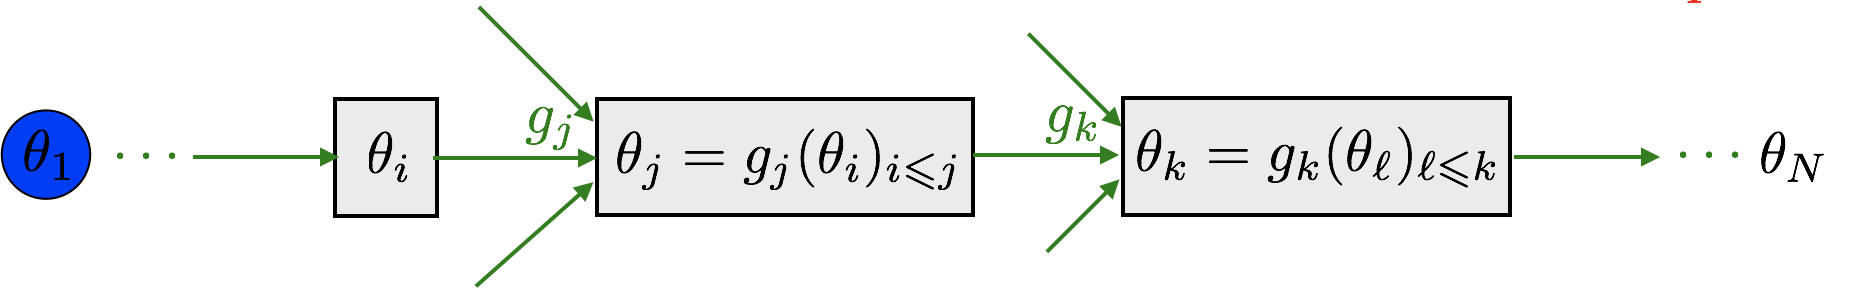
\includegraphics[width=.7\linewidth]{auto-diff/dag-element}}
\hbox{}\vspace{3mm}\hbox{}
\fbox{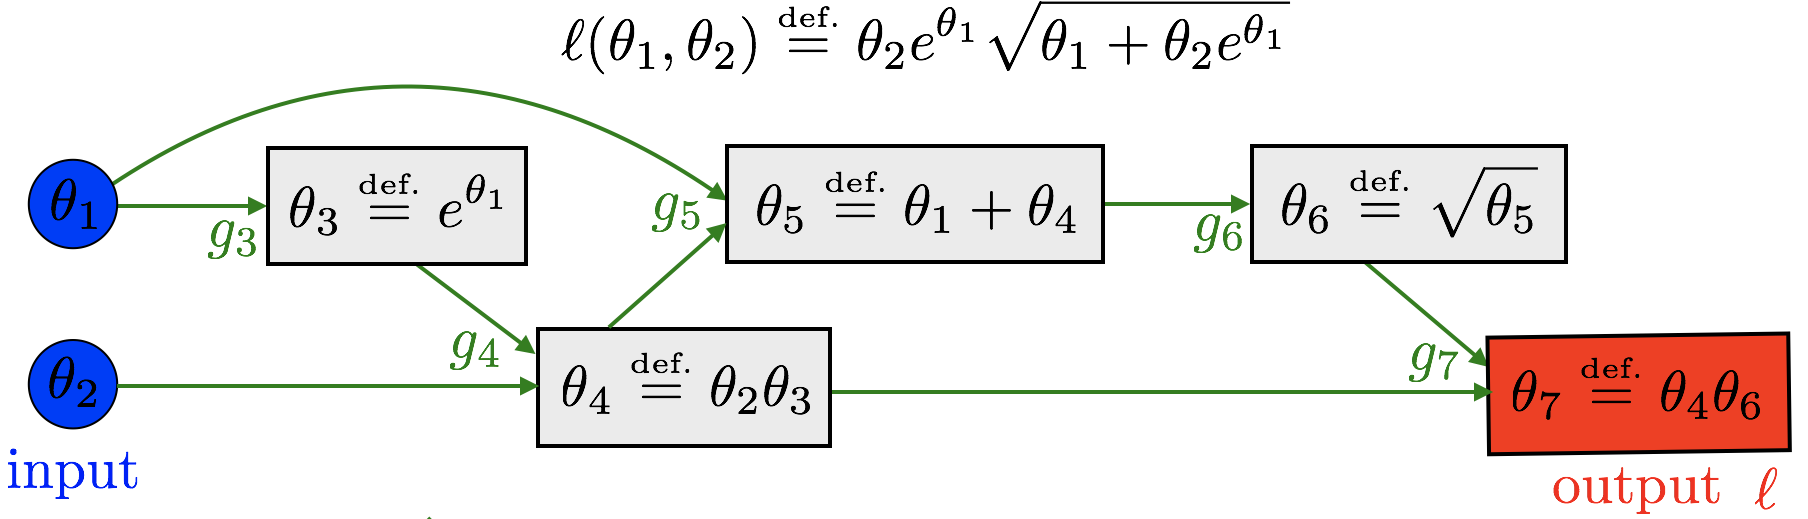
\includegraphics[width=.7\linewidth]{auto-diff/dag-example}}
\caption{\label{fig-dag-example}
Top: elementary component of the DAG computational graph. 
Bottom: example of DAG computational graph.
}
\end{figure}


One can generalize the idea above to differentiate automatically any function which can be implemented on a computer. What is even more surprising is that the computational cost is the same as the one of evaluating the function itself. This fundamental computational fact (that gradient evaluation and function evaluation have the same computational cost) is not so well known, but is of paramount practical interest when it comes to differentiating complicated recursive functions. We will apply it in a very simple setup for deep-architectures, but it can be applied to much more involved computational architectures. 

Note that this results only applies for function which output scalar values. For functions which output vector values, one can of course re-use this idea for each output, but this is in general vastly sub-optimal, because it ignore the redundancy between the computation of each output. The determination of optimal strategy in this case is known to be NP-hard. This include for instance the computation of the Hessian of a scalar valued function (since it corresponds to the differentiation of the gradient, which is itself a vector-valued function). Fortunately, for machine learning application, one is often interested in differentiating only empirical losses functions, which as scalar valued.

%%%%
\paragraph{Forward pass as a DAG traversal.}

The crux of this idea is that the computational flow of any computable function $\ell$ can be represented as a directed acyclic graph. 
%
We denote $(\th_i)_{i=1}^R$ the set of all scalar variables (input, output and intermediary) manipulated by the computational program.
%
Without loss of generality, we impose that the first variable $(\th_1,\ldots,\th_M)$ are the $M$ input variables, while the last $\th_R$ is the output variable. The function to be computed is thus of the form 
\eq{
	\th_R = \ell( \th_1,\ldots,\th_M )
}
where $\ell : \RR^M \rightarrow \RR$ is broken in $R-M+1$ intermediate steps corresponding to all the remaining variable $(\th_i)_{M < i < R}$. 
%
The successive execution of the program defines an ordering of all the intermediate variables, so that, after initializing the input variables $(\th_1,\ldots,\th_M)$, the forward pass computes the value of $\th_r$ for $r=M+1,\ldots,R$ as
\eq{
	\th_r = g_r( \th_{\pi(r)} )
}
for some scalar valued function $g_r : \RR^{|\pi(r)|} \rightarrow \RR$, where $\pi(r) \subset \{1,\ldots,r-1\}$ is the set of ``parent'' node of $r$ in a directed acyclic graph (DAG).  Figure~\ref{fig-dag-example} shows an example of such a computational DAG.


From a symbolic computation point of view, variables $\th_j$ (for $j>M$) in the graph can be interpreted either as variables (i.e. which can be assigned scalar values) and functions depending on input variables $\th_m$ for $m \leq M$. 
% 
The beauty of this DAG representation is that one can also view $\th_j$ as depending on any other intermediate variable $\th_i$ as long as $i<j$. 

%%%%
\paragraph{Direct mode auto-diff.}

The goal is to compute the gradient vector, which reads
\eq{
	\nabla \ell =  \pa{ \pd{\th_L}{\th_m} }_{m=1}^M. 
}
The naive way to comput this gradient vector would thus be to compute for each of the $M$ input variable $\th_m$ the differential $\pd{\th_j}{\th_m}$ of all function $\th_j$ with respect to $\th_m$. Without loss of generality, we consider $m=1$. This can be achieved by using the standard chain rule
\eql{\label{eq-chain-rule-forward}
	\pd{\th_j}{\th_1} = \sum_{i \in \pi(j)} \pd{\th_j}{\th_i} \pd{\th_i}{\th_1}.
}
Here the multipliers involved are actually differential of the elementary functions
\eq{
	\pd{\th_j}{\th_i} = \partial_i g_j
} 
Note that this writing is abusive, since $\pd{\th_j}{\th_i}$ really means that in practice such a differential is evaluated assuming all the variable $(\th_r)_{r<j}$ on which the function  $\th_j$ depends are defined to their respective value (which have been computed by the forward pass, which here can be run in parallel to the forward DAG traversal).

By traversing forward the DAG, iterating this formula compute all the derivative, and in particular $\pd{\th_j}{\th_1}$ and in particular $\nabla \ell_1 = \pd{\th_L}{\th_1}$. 
%
This approach, while being the most natural, is however vastly sub-optimal because its complexity is $M$ times the one of the evaluation of the function. 

%%%%
\paragraph{Reverse mode auto-diff.}

Instead of computing the quantities $(\pd{\th_j}{\th_1})_j$, a radically different approach consists in rather computing the quantities $\pd{\th_L}{\th_j} = (\nabla \ell)_j$. In place of the ``forward'' chain rule, one needs to the backward one
\eql{\label{eq-chain-rule-forward}
	\pd{\th_R}{\th_j} = \sum_{j \in \pi(k)} \pd{\th_N}{\th_k} \pd{\th_k}{\th_j}.
}
Note that here the summation is done over $k$ which are ``child'' of $j$ in the DAG. Here the multiplier appearing in the formula are differential of the elementary function since $\pd{\th_k}{\th_j} = \partial_j g_k$. 
%
The main interest of this reverse recursion~\eqref{eq-chain-rule-forward} with respect to the direct one~\eqref{eq-chain-rule-forward} is that it only needs to be run once, so that the overall complexity is the same as the one of the forward pass to compute the function itself. 

Figure~\ref{fig-fwdbwd} recap the two passes of the reverse mode automatic differentiation method.

\begin{figure}
\centering
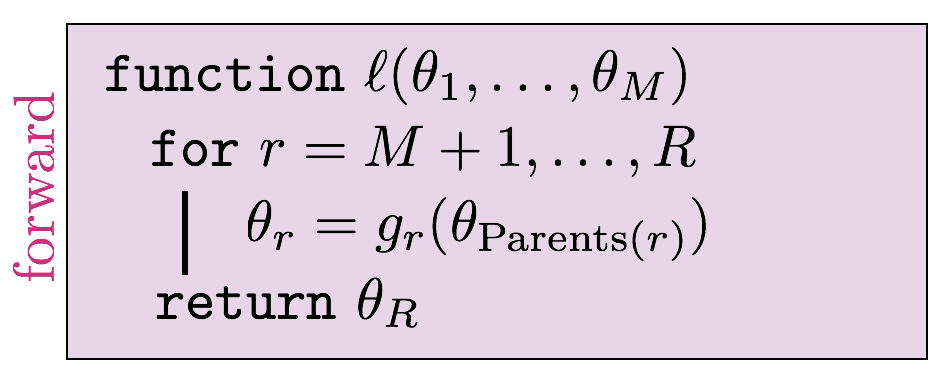
\includegraphics[width=.4\linewidth]{auto-diff/forward}
\qquad
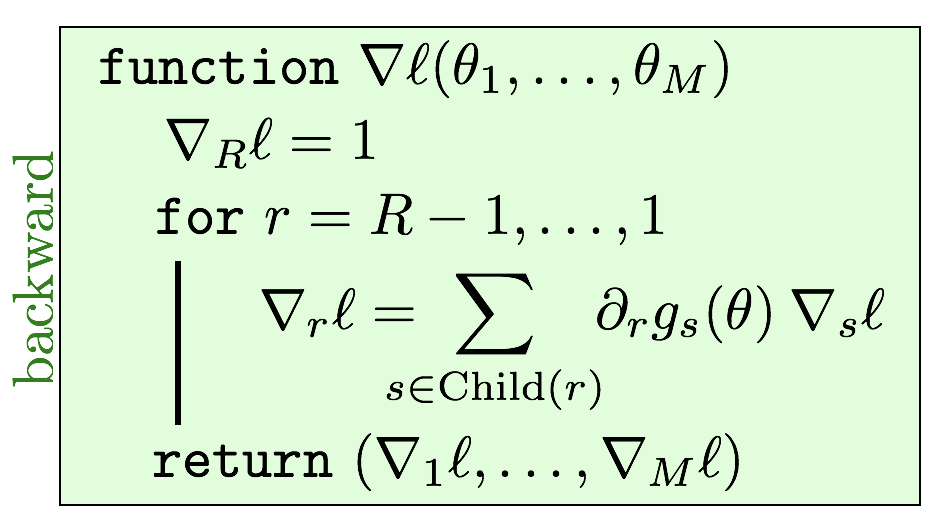
\includegraphics[width=.4\linewidth]{auto-diff/backward}
\caption{\label{fig-fwdbwd}
Recap of the two step of the automatic differentiation procedure.
}
\end{figure}

The main bottleneck of this backward automatic differentiation technic is the memory consumption. Indeed, since all intermediate results needs to be computed and stored explicitly before applying the backward pass, memory grows proportionally to execution time. This can be unacceptable for very large machine learning model. Fortunately, it is possible to trade time vs. memory and only keep track of a fraction of intermediate results, and retrieve the missing result locally by small forward passes. Doing this approach recursively allows to only have a logarithmic overhead in term of both time and memory, showing the vast superiority of automatic differentiation method with respect to any other alternative for differentiation. We could not insist more on the crucial importance and impact of this class of technics on modern data science. 

%%%%%%%%%%%%%%%%%%%%%%%%%%%%%%%%%%%%%%%%%%%%%%%%%%%%%%%%%%%%%%%%%%%%%%%%
%%%%%%%%%%%%%%%%%%%%%%%%%%%%%%%%%%%%%%%%%%%%%%%%%%%%%%%%%%%%%%%%%%%%%%%%
%%%%%%%%%%%%%%%%%%%%%%%%%%%%%%%%%%%%%%%%%%%%%%%%%%%%%%%%%%%%%%%%%%%%%%%%
\section{Deep Discriminative Models}
\label{sec-deepnet-discr}

%%%%%%%%%%%%%%%%%%%%%%%%%%%%%%%%%%%%%%%%%%
\subsection{General Deep Network Model}

Deep learning are estimator $f(x,\be)$ which are built as composition of simple building blocks.
%
In their simplest form (non-recursive), they corresponds to a simple linear computational graph as already defined in~\eqref{eq-simple-lin-dag} (without the loss $\Ll$), and we write this as
\eq{
	f(\cdot,\be) = f_{L-1}(\cdot,\be_1) \circ f_{L-2}(\cdot,\be_2) \circ \ldots \circ f_{0}(\cdot,\be_0)
}
where $\be=(\be_0,\ldots,\be_{L-1})$ is the set of parameters, and 
\eq{
	f_{\ell}(\cdot,\be_2) : \RR^{n_\ell} \rightarrow \RR^{n_{\ell+1}}
}
%
While it is possible to consider more complicated architecture (in particular recurrent one), we restrict here out attention to these simple linear graph computation structures (so-called feedforward networks).

The supervised learning of these parameters $\be$ is usually done by empirical risk minimization~\eqref{eq-erm-param} using SGD-type methods as explained in Section~\ref{sec-stochastic-optim}. Note that this results in highly non-convex optimization problem. In particular, strong convergence guarantees such as Theorem~\ref{thm-conv-sgd} do not hold anymore, and only weak convergence (toward stationary points) holds. SGD type technics are however found to work surprisingly well in practice, and it now believe that the success of these deep-architecture approaches (in particular the ability of these over-parameterized model to generalize well) are in large part due to the dynamics of the SGD itself, which induce an implicit regularization effect. 

For these simple linear architecture, the gradient of the ERM loss~\eqref{eq-grad-formula} can be computed using the reverse mode computation detailed in Section~\ref{sec-reversemode-simple}. In particular, in the context of deep learning, the formula~\eqref{eq-backprop}. One should however keep in mind that for more complicated (e.g. recursive) architecture, such a simple formula is not anymore available, and one should resort to reverse mode automatic differentiation (see Section~\ref{sec-reverse-mode}), which, while being conceptually simple, is actually implementing possibly highly non-trivial and computationally optimal recursive differentiation. 

In most successful applications of deep-learning, each computational block $f_{\ell}(\cdot,\be_\ell)$ is actually very simple, and is the composition of 
\begin{rs}
	\item an affine map, $B_\ell \cdot + b_\ell$ with a matrix $B_\ell \in \RR^{n_\ell \times \tilde n_{\ell}}$ and a vector $b_\ell \in \RR^{\tilde n_\ell}$ parametrized (in most case linearly) by $\be_\ell$, 
	\item a fixed (not depending on $\be_\ell$) non-linearity $\la_\ell : \RR^{\tilde n_{\ell}} \rightarrow \RR^{n_{\ell+1}}$
\end{rs}
which we write as
\eql{\label{eq-struc-layer}
	\foralls x_\ell \in \RR^{n_\ell}, \quad
	f_{\ell}(x_\ell,\be_\ell) = \la_\ell(  B_\ell x_\ell + b_\ell ) \in \RR^{n_{\ell+1}}. 
}
In the simplest case, the so-called ``fully connected'', one has $(B_\ell,b_\ell)=\be_\ell$, i.e. $B_\ell$ is a full matrix and its entries (together with the bias $b_\ell$) are equal to the set of parameters $\be_\ell$. 
%
Also in the simplest case,s $\la_\ell$ is a pointwise non-linearity $\la_\ell(z)=(\tilde\la_\ell(z_k))_k$, where $\tilde\la_\ell : \RR \rightarrow \RR$ is non-linear. The most usual choice are the rectified linear unit (ReLu) $\tilde\la_\ell(s)=\max(s,0)$ and the sigmoid $\tilde\la_\ell(s)=\th(s) = (1+e^{-s})^{-1}$.

An issue with this fully connected setting is that the number of parameters is too large to be applicable to large scale data such as images. Furthermore, it ignore any prior knowledge about the data, such as for instance some invariance. This is addressed in more structured architecture, such as for instance convolutional network detailed in Section~\ref{sec-cnn}. 


%%%%%%%%%%%%%%%%%%%%%%%%%%%%%%%%%%%%%%%%%%
\subsection{Perceptron and Shallow Models}

Before going on with the description of deep architecture, let us re-interpret the logistic classification method detailed in Sections~\ref{sec-two-class-logit} and~\ref{sec-multiclass-logit}.

The two-class logistic regression model~\eqref{eq-two-class-logit-model} is equal to a single layer ($L=1$) network of the form~\eqref{eq-struc-layer} where 
\eq{
	B_0 x = \dotp{x}{\be}
	\qandq
	\tilde\la(s) = \th(s).
}
In this case, the ERM optimization is of course a convex program. 

% The multi-class model 



%%%%%%%%%%%%%%%%%%%%%%%%%%%%%%%%%%%%%%%%%%
\subsection{Convolutional Neural Networks}
\label{sec-cnn}



%%%%%%%%%%%%%%%%%%%%%%%%%%%%%%%%%%%%%%%%%%%%%%%%%%%%%%%%%%%%%%%%%%%%%%%%
%%%%%%%%%%%%%%%%%%%%%%%%%%%%%%%%%%%%%%%%%%%%%%%%%%%%%%%%%%%%%%%%%%%%%%%%
%%%%%%%%%%%%%%%%%%%%%%%%%%%%%%%%%%%%%%%%%%%%%%%%%%%%%%%%%%%%%%%%%%%%%%%%
\section{Deep Generative Models}
\label{sec-deepnet-gen}


%%%%%%%%%%%%%%%%%%%%%%%%%%%%%%%%%%%%%%%%%%
\subsection{Density Fitting}

%%%
\paragraph{Fitting and MLE}

%%%
\paragraph{Generative Models}

%%%%%%%%%%%%%%%%%%%%%%%%%%%%%%%%%%%%%%%%%%
\subsection{Auto-encoders}

%%%%%%%%%%%%%%%%%%%%%%%%%%%%%%%%%%%%%%%%%%
\subsection{GANs}